%%
%% Beginning of file 'sample61.tex'
%%
%% Modified 2016 September
%%
%% This is a sample manuscript marked up using the
%% AASTeX v6.1 LaTeX 2e macros.
%%
%% AASTeX is now based on Alexey Vikhlinin's emulateapj.cls 
%% (Copyright 2000-2015).  See the classfile for details.

%% AASTeX requires revtex4-1.cls (http://publish.aps.org/revtex4/) and
%% other external packages (latexsym, graphicx, amssymb, longtable, and epsf).
%% All of these external packages should already be present in the modern TeX 
%% distributions.  If not they can also be obtained at www.ctan.org.

%% The first piece of markup in an AASTeX v6.x document is the \documentclass
%% command. LaTeX will ignore any data that comes before this command. The 
%% documentclass can take an optional argument to modify the output style.
%% The command below calls the preprint style  which will produce a tightly 
%% typeset, one-column, single-spaced document.  It is the default and thus
%% does not need to be explicitly stated.
%%
%%
%% using aastex version 6.1
\documentclass[twocolumn]{aastex61}

%% The default is a single spaced, 10 point font, single spaced article.
%% There are 5 other style options available via an optional argument. They
%% can be envoked like this:
%%
%% \documentclass[argument]{aastex61}
%% 
%% where the arguement options are:
%%
%%  twocolumn   : two text columns, 10 point font, single spaced article.
%%                This is the most compact and represent the final published
%%                derived PDF copy of the accepted manuscript from the publisher
%%  manuscript  : one text column, 12 point font, double spaced article.
%%  preprint    : one text column, 12 point font, single spaced article.  
%%  preprint2   : two text columns, 12 point font, single spaced article.
%%  modern      : a stylish, single text column, 12 point font, article with
%% 		  wider left and right margins. This uses the Daniel
%% 		  Foreman-Mackey and David Hogg design.
%%
%% Note that you can submit to the AAS Journals in any of these 6 styles.
%%
%% There are other optional arguments one can envoke to allow other stylistic
%% actions. The available options are:
%%
%%  astrosymb    : Loads Astrosymb font and define \astrocommands. 
%%  tighten      : Makes baselineskip slightly smaller, only works with 
%%                 the twocolumn substyle.
%%  times        : uses times font instead of the default
%%  linenumbers  : turn on lineno package.
%%  trackchanges : required to see the revision mark up and print its output
%%  longauthor   : Do not use the more compressed footnote style (default) for 
%%                 the author/collaboration/affiliations. Instead print all
%%                 affiliation information after each name. Creates a much
%%                 long author list but may be desirable for short author papers
%%
%% these can be used in any combination, e.g.
%%
%% \documentclass[twocolumn,linenumbers,trackchanges]{aastex61}

%% AASTeX v6.* now includes \hyperref support. While we have built in specific
%% defaults into the classfile you can manually override them with the
%% \hypersetup command. For example,
%%
%%\hypersetup{linkcolor=red,citecolor=green,filecolor=cyan,urlcolor=magenta}
%%
%% will change the color of the internal links to red, the links to the
%% bibliography to green, the file links to cyan, and the external links to
%% magenta. Additional information on \hyperref options can be found here:
%% https://www.tug.org/applications/hyperref/manual.html#x1-40003

%% If you want to create your own macros, you can do so
%% using \newcommand. Your macros should appear before
%% the \begin{document} command.
%%
\newcommand{\vdag}{(v)^\dagger}
\newcommand\aastex{AAS\TeX}
\newcommand\latex{La\TeX}
\newcommand{\sm}{M_\odot}
\newcommand{\sr}{R_\odot}

%% Reintroduced the \received and \accepted commands from AASTeX v5.2
\received{\today}
\revised{}
\accepted{}
%% Command to document which AAS Journal the manuscript was submitted to.
%% Adds "Submitted to " the arguement.
\submitjournal{ApJ}

%% Mark up commands to limit the number of authors on the front page.
%% Note that in AASTeX v6.1 a \collaboration call (see below) counts as
%% an author in this case.
%
%\AuthorCollaborationLimit=3
%
%% Will only show Schwarz, Muench and "the AAS Journals Data Scientist 
%% collaboration" on the front page of this example manuscript.
%%
%% Note that all of the author will be shown in the published article.
%% This feature is meant to be used prior to acceptance to make the
%% front end of a long author article more manageable. Please do not use
%% this functionality for manuscripts with less than 20 authors. Conversely,
%% please do use this when the number of authors exceeds 40.
%%
%% Use \allauthors at the manuscript end to show the full author list.
%% This command should only be used with \AuthorCollaborationLimit is used.

%% The following command can be used to set the latex table counters.  It
%% is needed in this document because it uses a mix of latex tabular and
%% AASTeX deluxetables.  In general it should not be needed.
%\setcounter{table}{1}

%%%%%%%%%%%%%%%%%%%%%%%%%%%%%%%%%%%%%%%%%%%%%%%%%%%%%%%%%%%%%%%%%%%%%%%%%%%%%%%%
%%
%% The following section outlines numerous optional output that
%% can be displayed in the front matter or as running meta-data.
%%
%% If you wish, you may supply running head information, although
%% this information may be modified by the editorial offices.
\shorttitle{iPTF16abc}
\shortauthors{Cao et al.}
%%
%% You can add a light gray and diagonal water-mark to the first page 
%% with this command:
\watermark{DRAFT}
%% where "text", e.g. DRAFT, is the text to appear.  If the text is 
%% long you can control the water-mark size with:
%  \setwatermarkfontsize{dimension}
%% where dimension is any recognized LaTeX dimension, e.g. pt, in, etc.
%%
%%%%%%%%%%%%%%%%%%%%%%%%%%%%%%%%%%%%%%%%%%%%%%%%%%%%%%%%%%%%%%%%%%%%%%%%%%%%%%%%

%%%%%%%%%%%%%%%%%%%%%%%%%%%%%%%%%%%%%%%%%%%%%%%%%%%%%%%%%%%%%%%%%%%%%%%%%%%%%%%%
%%
%% The following section defines new commands for comments from co-authors
%%
\newcommand{\ycao}[1]{{\color{red} ycao: {#1}}}
\newcommand{\amiller}[1]{{\color{blue} amiller: {#1}}}
%%
%%%%%%%%%%%%%%%%%%%%%%%%%%%%%%%%%%%%%%%%%%%%%%%%%%%%%%%%%%%%%%%%%%%%%%%%%%%%%%%%

%% This is the end of the preamble.  Indicate the beginning of the
%% manuscript itself with \begin{document}.

\begin{document}

\title{Optifcal Observations of an Extraordinarily Young Type Ia Supernova iPTF16abc}

%% LaTeX will automatically break titles if they run longer than
%% one line. However, you may use \\ to force a line break if
%% you desire. In v6.1 you can include a footnote in the title.

%% A significant change from earlier AASTEX versions is in the structure for 
%% calling author and affilations. The change was necessary to implement 
%% autoindexing of affilations which prior was a manual process that could 
%% easily be tedious in large author manuscripts.
%%
%% The \author command is the same as before except it now takes an optional
%% arguement which is the 16 digit ORCID. The syntax is:
%% \author[xxxx-xxxx-xxxx-xxxx]{Author Name}
%%
%% This will hyperlink the author name to the author's ORCID page. Note that
%% during compilation, LaTeX will do some limited checking of the format of
%% the ID to make sure it is valid.
%%
%% Use \affiliation for affiliation information. The old \affil is now aliased
%% to \affiliation. AASTeX v6.1 will automatically index these in the header.
%% When a duplicate is found its index will be the same as its previous entry.
%%
%% Note that \altaffilmark and \altaffiltext have been removed and thus 
%% can not be used to document secondary affiliations. If they are used latex
%% will issue a specific error message and quit. Please use multiple 
%% \affiliation calls for to document more than one affiliation.
%%
%% The new \altaffiliation can be used to indicate some secondary information
%% such as fellowships. This command produces a non-numeric footnote that is
%% set away from the numeric \affiliation footnotes.  NOTE that if an
%% \altaffiliation command is used it must come BEFORE the \affiliation call,
%% right after the \author command, in order to place the footnotes in
%% the proper location.
%%
%% Use \email to set provide email addresses. Each \email will appear on its
%% own line so you can put multiple email address in one \email call. A new
%% \correspondingauthor command is available in V6.1 to identify the
%% corresponding author of the manuscript. It is the author's responsibility
%% to make sure this name is also in the author list.
%%
%% While authors can be grouped inside the same \author and \affiliation
%% commands it is better to have a single author for each. This allows for
%% one to exploit all the new benefits and should make book-keeping easier.
%%
%% If done correctly the peer review system will be able to
%% automatically put the author and affiliation information from the manuscript
%% and save the corresponding author the trouble of entering it by hand.

\correspondingauthor{Yi Cao}
\email{ycao16@uw.edu}

\author[0000-0002-8036-8491]{Yi Cao}
\affil{eScience Institute and Astronomy Department, University of Washington,
  Seattle, WA 98195}

\author{Friends}
\affil{the intermediate Palomar Transient Factory}

%% Note that the \and command from previous versions of AASTeX is now
%% depreciated in this version as it is no longer necessary. AASTeX 
%% automatically takes care of all commas and "and"s between authors names.

%% AASTeX 6.1 has the new \collaboration and \nocollaboration commands to
%% provide the collaboration status of a group of authors. These commands 
%% can be used either before or after the list of corresponding authors. The
%% argument for \collaboration is the collaboration identifier. Authors are
%% encouraged to surround collaboration identifiers with ()s. The 
%% \nocollaboration command takes no argument and exists to indicate that
%% the nearby authors are not part of surrounding collaborations.

%% Mark off the abstract in the ``abstract'' environment. 
\begin{abstract}

  We report the discovery of an extraordinarily young Type Ia supernova,
  iPTF16abc, by the intermediate Palomar Transient Factory. Our first
  observation was made only $0.18$~d after the onset of the
  supernova explosion. Our analysis shows that the early emission from iPTF16abc is dominated by radioactive decay, and that contributions from supernova shock breakout or the ejecta colliding with a stellar companion are minimal. The combination of (i) a fast initial rise, (ii) the
  early exponential decline in the photospheric velocity, and (iii) the significant presence of ionized carbon in the earliest spectra together provide
  evidence for the strong mixing of radioactive elements in the supernova ejecta. \amiller{There should be something about dark times/lack of dark time for this SN in the abstract.}

\end{abstract}

%% Keywords should appear after the \end{abstract} command. 
%% See the online documentation for the full list of available subject
%% keywords and the rules for their use.
\keywords{methods: observational --- supernovae: individual (iPTF16abc)}

%% From the front matter, we move on to the body of the paper.
%% Sections are demarcated by \section and \subsection, respectively.
%% Observe the use of the LaTeX \label
%% command after the \subsection to give a symbolic KEY to the
%% subsection for cross-referencing in a \ref command.
%% You can use LaTeX's \ref and \label commands to keep track of
%% cross-references to sections, equations, tables, and figures.
%% That way, if you change the order of any elements, LaTeX will
%% automatically renumber them.

%% We recommend that authors also use the natbib \citep
%% and \citet commands to identify citations.  The citations are
%% tied to the reference list via symbolic KEYs. The KEY corresponds
%% to the KEY in the \bibitem in the reference list below. 

\section{Introduction}
\label{sec:intro}

Although Type Ia supernovae (SNe Ia) have been extensively used as
standardizable candles, their progenitors and explosion
physics are still debated (see a recent review by
\citealt{2014ARA&A..52..107M}). Extremely detailed
observations in the hours to days after explosion are one of the most promising avenues to further
constrain this problem.

While the shock breakout of a SN Ia occurs on a sub-second timescale,
the subsequent quasi-adiabatic expanding and cooling of the unbound
ejecta produces thermal emission that can be used to infer the
original size of the exploding star
\citep{2010ApJ...708..598P,2011ApJ...728...63R}. Comparing models of
this cooling emission to the earliest-phase data of SN~2011fe,
\citet{2012ApJ...744L..17B} concluded that the radius of the SN~2011fe progenitor is $\lesssim0.01\sr$, where $\sr$ is the solar
radius. Combining this size constraint and the measured ejecta mass to
derive the mean density of the progenitor star, we confirmed that the
progenitor star is compact and degenerate\ycao{Ref?}. \ycao{a transition is missing here - not sure how the second half of this paragraph relates to the first} Admittedly, due to the
initial small surface area of the progenitor star, the shock cooling
emission of a SN Ia decays drastically as the ejecta expands. Given
typical parameters for a SN Ia, this thermal emission is visible from
events up to $\sim 10\,\textrm{Mpc}$ within one day of their explosions.

SN Ia resulting from a white dwarf and non-degenerate companion, referred to as the single-degenerate progenitor, early-phase observations may detect excess emission due to the collision of the SN ejecta and the non-degenerate companion \citep{1973ApJ...186.1007W,2010ApJ...708.1025K}. This excess emission was first detected in iPTF14atg,  \citep{2015Natur.521..328C}, a low-velocity SN Ia with a significant and declining ultraviolet pulse detected within a
few days of the SN explosion. This signature is best interpreted as a
SN ejecta-companion collision. Many studies have searched for this excess emission, with most resulting in non-detections
\citep{2010ApJ...722.1691H,2011ApJ...741...20B,2012ApJ...744...38F,
  2012ApJ...744L..17B,2015Natur.521..332O,
  2013ApJ...778L..15Z,2015ApJ...799..106G,2016ApJ...826..144S,
  2015ApJS..221...22I}. An exception is SN2012cg, 
  as a blue excess in its early-phase light curve is attributed to an ejecta-companion collision in \citet{2016ApJ...820...92M} (though see \citealt{2016arXiv161007601S} for an alternative interpretation). 
With only $\sim 10\%$ of single-degenerate progenitors occupying the preferred binary geometry for us to see the collision
signatures, it is not surprising that there are few confirmed detections in the literature \ycao{ref?}. 

More commonly, the only observed light curve of a SN Ia is purely
powered by the radioactive decay of synthesized $^{56}$Ni. Since
$^{56}$Ni atoms are synthesized, mixed and deposited into different
layers inside the ejecta, the SN may experience a dark period after
the SN shock breakout and before the radioactive energy diffuses to
the photosphere \citep{2014ApJ...784...85P}. In the case of strong
mixing, $^{56}$Ni energy can reach the photosphere rapidly. As such,
the dark period is very short and the light curve shows a fast initial
rise. In the opposite case, it may take up to a couple of days for
the $^{56}$Ni energy to diffuse to the photosphere. The initial rise
of the light curve is then moderate \citep{2016ApJ...826...96P}. To
summarize, the initial rise of the light curve of a SN Ia conveys
information on distribution of synthesized $^{56}$Ni. 

In this paper, we report observations of an extraordinarily young SN
Ia iPTF16abc, which was discovered by the intermediate Palomar
Transient Factory on 2016 April $3.36$\footnote{all times in this
  paper are in UTC.} at $\textrm{R.A.}=13^h34^m45.49^s$,
$\textrm{Dec.}=+13^d51^m14.3^s$ (J2000) with a $g$-band magnitude of
$21.31\pm0.27$ \citep{2016PASP..128k4502C,2016ATel.8907....1M}. The
transient is spatially coincident with a tidal tail of the galaxy
NGC\,5221 at 100\,Mpc. No activity was detected at the same location
down to $g=22.1$\,mag on April $2.42$. Our spectroscopic follow-up
compaign classified iPTF16abc as a normal SN Ia
\citep{2016ATel.8909....1C}.

This paper is organized as follows: Section \ref{sec:obs} describes
photometric and spectroscopic observations of iPTF16abc. Section
\ref{sec:usual_staff} establishes that iPTF16abc is a normal SN Ia
in NGC\,5221. Section \ref{sec:first_light} analyzes the early
light curve and spectra.

\section{Observations}
\label{sec:obs}

\begin{figure*}[htb]
  \centering
  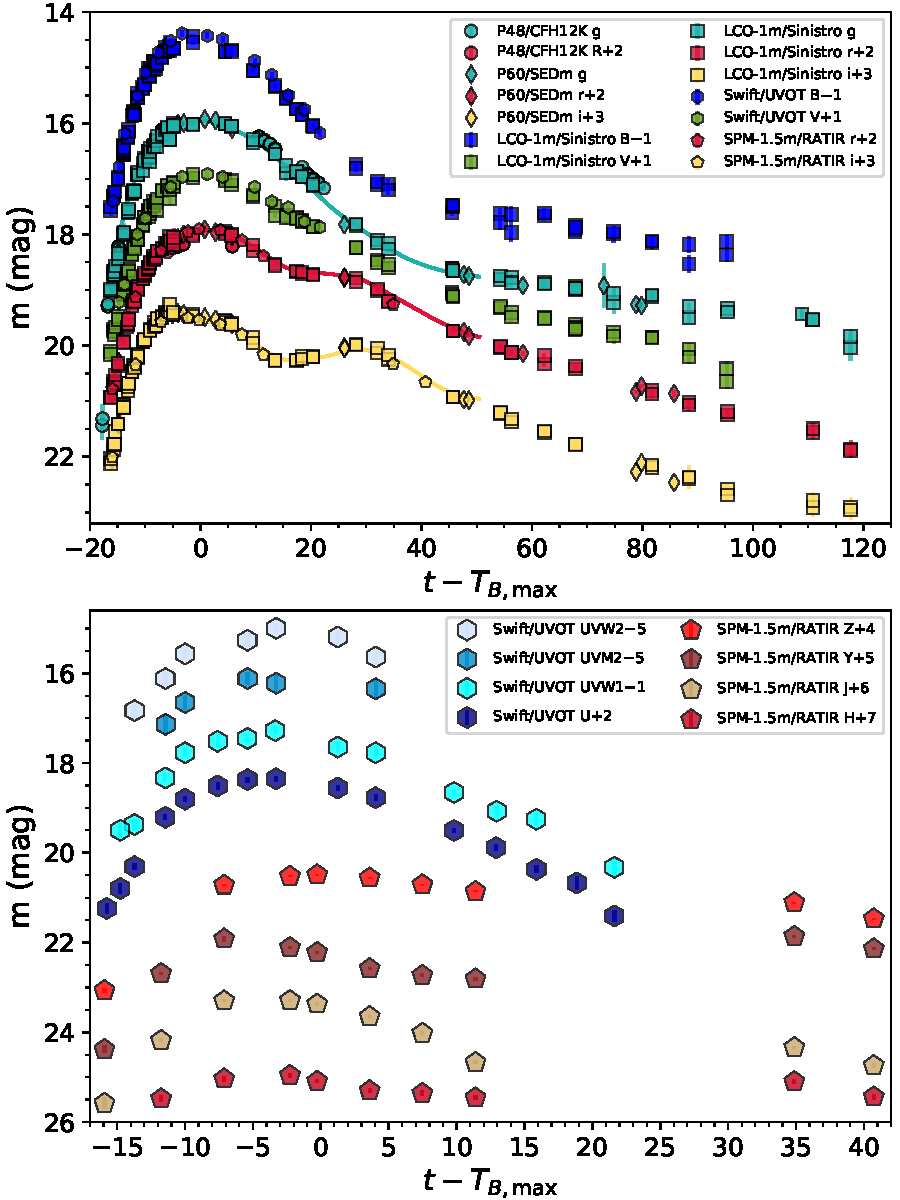
\includegraphics[width=0.95\textwidth]{lightcurve.pdf}
  \caption{Multi-band light curves of iPTF16abc are shown. Filters are
    denoted by different colors and observation instruments by
    different markers. The $t_{max}$ time is the B-band maximum
    determined by SALT2 (Section \ref{sec:classification}). The solid
    curves are best-fit results from SALT2. The black ticks near the
    top of the figure shows epochs of spectroscopic observations.}
  \label{fig:lightcurve}
\end{figure*}

As part of the iPTF transient survey in the 2016 spring quarter, the
field of iPTF16abc was observed in $g$- or $R$-band every night by the
CFH12K camera \citep{2000SPIE.3965...58S} on the 48-inch telescope at
Palomar Observatory (P48). The images were processed by the IPAC image
subtraction and discovery pipeline which subtracts off the background
galaxy light with stacked pre-SN images and performs forced
point-spread-function (PSF) photometry at the location of the SN. The
photometry is then calibrated to the PTF photometric catalog
\citep{2012PASP..124..854O}.

After discovery, we utilized the rainbow camera of the SED Machine
(\ycao{REF}) mounted on the 60-inch telescope at Palomar Observatory
(P60) to undertake photometric observations in $g$, $r$ and $i$
filters. The image differencing against the archival SDSS images and
forced PSF photometry on the subtracted images were performed by the
Fremling Automated Pipeline \citep{2016A&A...593A..68F}. The
photometry is also calibrated to the SDSS catalog \ycao{which DR?}.

Las Cambres Observatory Global Network (LCOGT) also carry out
photometric observations in the \textit{BVgri} filters with its 1-m
telescope network.  PSF photometry was measured on these images using
the \texttt{lcogtsnpipe} pipeline \citep{2016MNRAS.459.3939V}. The
\textit{BV} magnitudes are calibrated to the Fourth USNO CCD
Astrograph Catalog \citep{2013AJ....145...44Z}, and the \textit{gri}
magnitudes are calibrated to SDSS Data Release 6
\citep{2008ApJS..175..297A}.

In space, \textit{Swift} observed iPTF16abc for 14 epochs, covering
from the very early phase to the post-peak phase. Aperture photometry
are carried out on the images taken by its Ultraviolet-Optical
Telescope (UVOT) with the usual procedures in the HEASoft and
corrected for the coincident loss and aperture loss. The image counts
are converted to physical fluxes using the latest calibration
\citep{2011AIPC.1358..373B}. No pre-SN UVOT image at the SN location
is available in the \textit{Swift} archive.  Visual inspection to the
UVOT images suggests that the background galaxy light in the UVOT
filters is probably negligible. No X-ray emission was detected at the
location of the SN by the X-ray Telescope (XRT) in any of these
epochs.

The multi-color light curves of iPTF16abc are illustrated in Figure
\ref{fig:lightcurve}.  For convenience, magnitudes in \textit{all}
filters are in the AB system with a zero point of $3631$\,Jy.

Spectroscopic observations of iPTF16abc were undertaken with a variety
of telescopes and instruments in multiple epochs spanning from a
couple of days after explosion to two months after its maximum. An
observing log is listed in Table \ref{tab:spec_obs_log}. Data
reduction is undertaken with usual routines in IDL/Python. Except for
the high-resolution spectra obtained by VLT instruments, the optical
spectral evolution of iPTF16abc is illustrated in Figure
\ref{fig:spec_seq}.

\begin{deluxetable*}{cccccc}
  \tablecaption{Spectroscopic observations of iPTF16abc \label{tab:spec_obs_log}}
  \tablehead{
    \colhead{Observation MJD} & \colhead{SN phase} & \colhead{Telescope} &
    \colhead{Instrument} & \colhead{Wavelength Coverage (\AA)}
  }
  \startdata
  $57483.26$ & $-16.4$ & DCT & DeVeny\tablenotemark{1} & $3301$--$7499$ \\
  $57483.88$ & $-15.8$ & Gemini-North & GMOS\tablenotemark{2} & $3800$--$9200$ \\
  $57484.51$ & $-15.1$ & Keck-II & DEIMOS\tablenotemark{3} & $5500$--$8099$ \\
  $57486.51$ & $-13.1$ & Keck-II & DEIMOS\tablenotemark{3} & $5500$--$8099$ \\
  $57488.38$ & $-11.3$ & Keck-I & LRIS\tablenotemark{4} & $3055$--$10411$ \\
  $57489.51$ & $-10.1$ & LCOGT-2m & FLOYDS\tablenotemark{5} & $3301$--$8999$ \\
  $57490.40$ & $ -9.3$ & LCOGT-2m & FLOYDS\tablenotemark{5} & $3301$--$9999$ \\
  $57491.55$ & $ -8.1$ & LCOGT-2m & FLOYDS\tablenotemark{5} & $3300$--$9998$ \\
  $57492.20$ & $ -7.5$ & VLT & X-shooter\tablenotemark{6} & $3300$--$24550$ \\
  $57494.00$ & $ -5.7$ & VLT & UVES\tablenotemark{7} & \\
  $57503.32$ & $ +3.7$ & LCOGT-2m & FLOYDS\tablenotemark{5} & $3300$--$9999$ \\
  $57506.00$ & $ +6.3$ & NOT & ALFOSC\tablenotemark{8} & $3602$--$8098$ \\
  $57508.27$ & $ +8.6$ & LCOGT-2m & FLOYDS\tablenotemark{5} & $3301$--$9999$ \\
  $57518.42$ & $+18.8$ & Keck-I & LRIS\tablenotemark{4} & $3071$--$10208$ \\
  $57520.03$ & $+20.4$ & VLT & X-shooter\tablenotemark{6} & $3300$--$24789$ \\
  $57529.40$ & $+29.8$ & LCOGT-2m & FLOYDS\tablenotemark{5} & $4000$--$8998$ \\
  $57542.41$ & $+42.8$ & LCOGT-2m & FLOYDS\tablenotemark{5} & $4000$--$8998$ \\
  $57550.40$ & $+50.8$ & LCOGT-2m & FLOYDS\tablenotemark{5} & $4001$--$8999$ \\
  $57562.38$ & $+62.7$ & LCOGT-2m & FLOYDS\tablenotemark{5} & $4800$--$9300$ \\
  \enddata
  \tablenotetext{1}{The Deveny Spectrograph \citep{2014SPIE.9147E..2NB}}
  \tablenotetext{2}{The Gemini Multi-Object Sectrograph \citep{2004PASP..116..425H}}
  \tablenotetext{3}{DEep Imaging Multi-Object Spectrograph \citep{2003SPIE.4841.1657F}}
  \tablenotetext{4}{Low-Resolution Imaging Spectrometer \citep{1995PASP..107..375O}}
  \tablenotetext{5}{FLOYDS \url{https://lco.global/observatory/instruments/floyds}}
  \tablenotetext{6}{X-shooter \citep{XShooter}}
  \tablenotetext{7}{Ultraviolet and Visual Echelle Spectrograph \citep{2000SPIE.4008..534D}}
  \tablenotetext{8}{The Andalucia Faint Object Spectrograph and Camera \url{http://www.not.iac.es/instruments/alfosc}}
\end{deluxetable*}

\begin{figure*}[!htb]
  \centering
  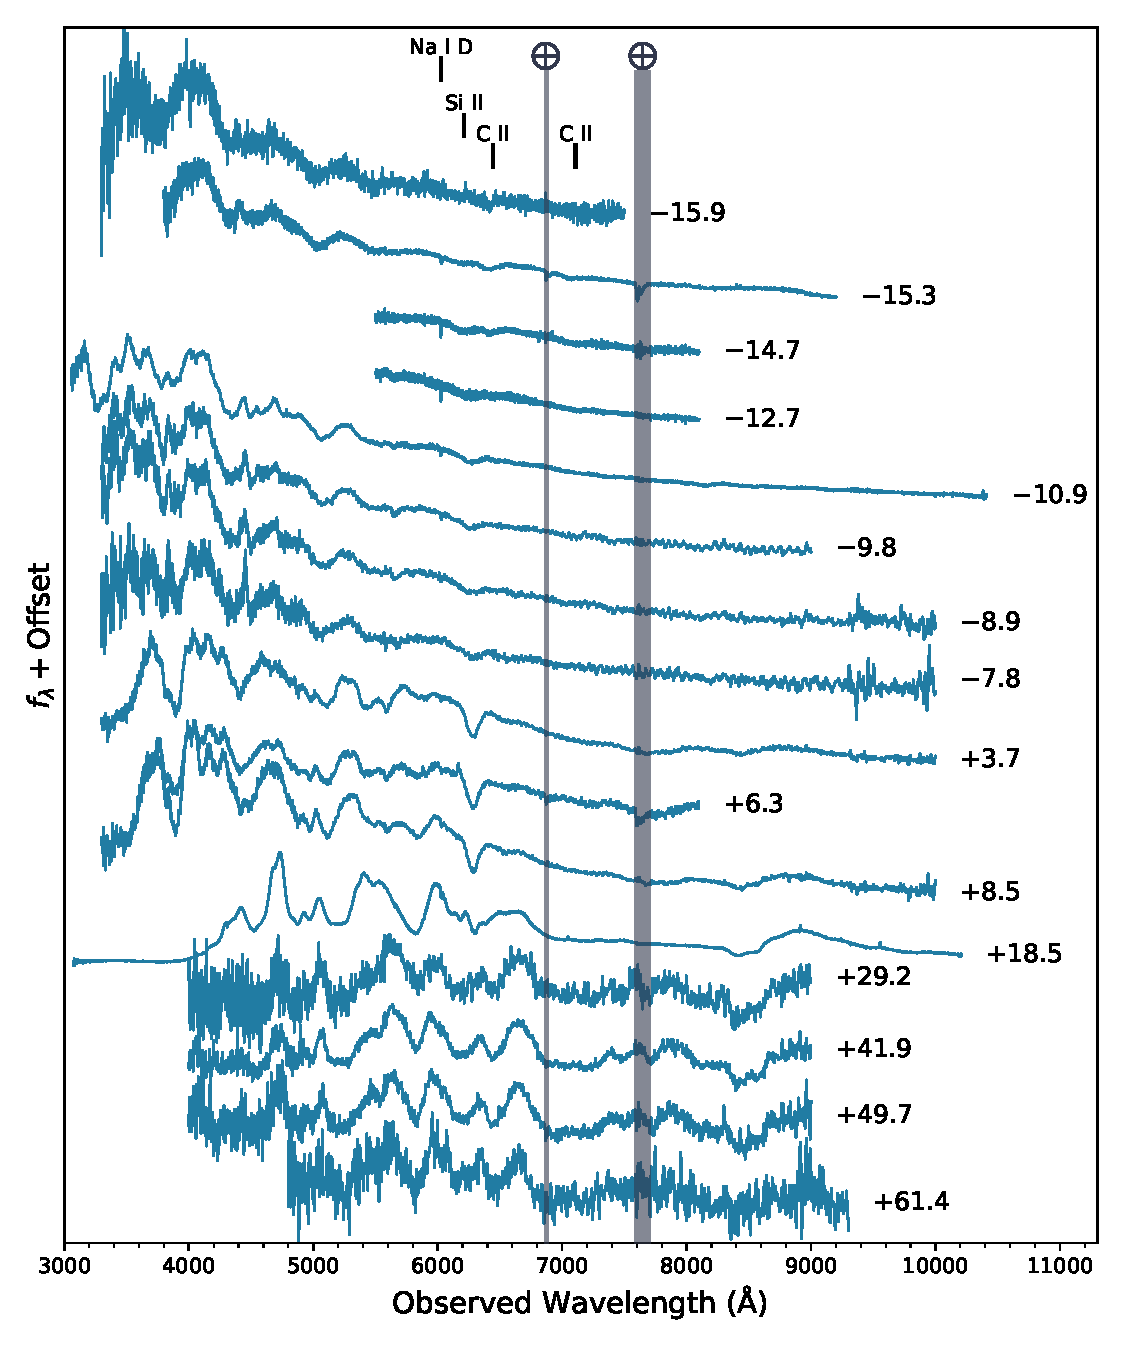
\includegraphics[width=1.0\textwidth]{spectra.pdf}
  \caption{Low-resolution spectra of iPTF16abc are shown in the
    chronical orders. In order for better illustration, each spectrum
    is normalized by the median flux value between $6,000$ and
    $7,000\,\textrm{\AA}$ and offset properly.  The phases in units of
    days are noted next to corresponding spectra. Telluric absorption
    bands are grayed out. The narrow \ion{Na}{1}\,D absorption is also
    highlighted in orange.}
  \label{fig:spec_seq}
\end{figure*}


\section{Reddening, Classification and Host Galaxy}
\label{sec:usual_staff}

\subsection{Reddening}
\label{sec:reddening}

The foreground Galactic extinctioin along the directionof iPTF16abc
has $E(B-V)=0.0279\,\textrm{mag}$ \citep{2011ApJ...737..103S}.

In the highest-resolution spectrum of iPTF16abc by UVES, individual
components of both \ion{Ca}{2}\,H$+$K and \ion{Na}{1}\,D doublets show
double-absorption profiles (Figure \ref{fig:narrow_features}),
indicating two sources of absorption along the line of sight. Fitting
two Gaussian kernels to each line of the \ion{Na}{1} doublet
simultaneously leads to redshifts of $0.02313820\pm0.00000032$ and
$0.02322408\pm0.00000033$. The total equivalent widths of the
\ion{Na}{1}\,D1 and D2 lines are $0.595\pm0.009\,\textrm{\AA}$ and
$0.609\pm0.008\,\textrm{\AA}$m, respectively. Using the empirical
relation between the equivalent width of \ion{Na}{1}\,D lines and
reddening $E(B-V)$ \citep{2012MNRAS.426.1465P}, we derive
$E(B-V)=0.361\pm0.025\textrm{mag}$. We caution that the empirical
relation has a quite large scatter.

In the X-shooter spectra of iPTF16abc, we also identify narrow
absorption features \ion{K}{1}\,7665\,\AA and 7699\,\AA at consistent
redshifts. However, the resolution of the X-shooter spectra is not
fine enough to resolve the double-absorption profiles of \ion{Ca}{2}
and \ion{Na}{1}. The X-shooter spectra do not show the diffusive
interstellar band at 5780\,\AA as well.  Albeit some debates (e.g.,
\citealt{2013ApJ...779...38P}), the $E(B-V)$ value derived from
\ion{Na}{1}\,D absorption provides the best estimate in the case of
iPTF16abc.

\begin{figure}[htb]
  \centering
  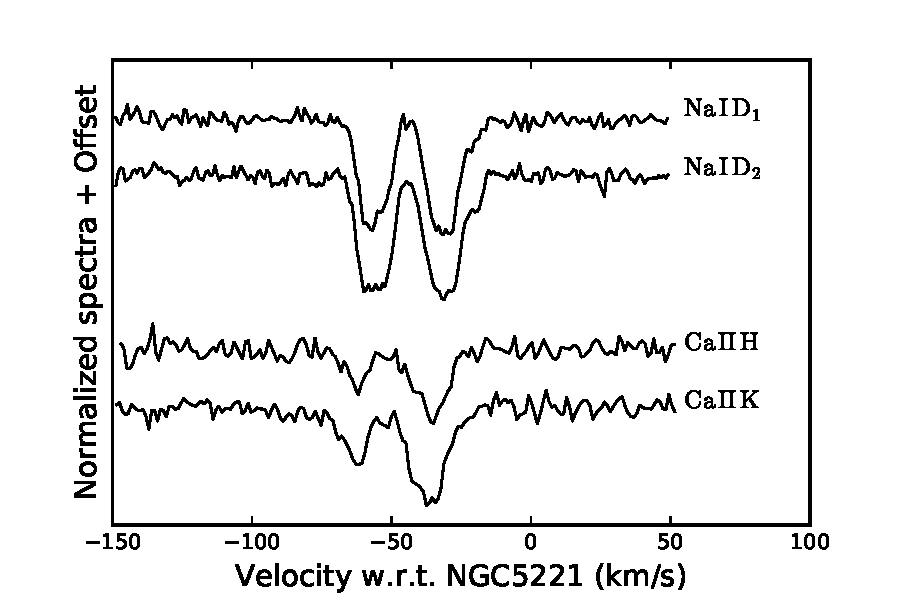
\includegraphics[width=0.45\textwidth]{narrow_abs_features.pdf}
  \caption{Narrow absorption lines of iPTF16abc are shown in this
    figure. The zero velocity corresponds to the redshift of the
    apparent host NGC\,5221.}
  \label{fig:narrow_features}
\end{figure}

The \ion{Na}{1}\,D doublet are seen in multiple spectra spanning
from pre-peak to post-peak phases. Despite the instrumental widening of
different instrument configurations, we do not detect obvious variation
in the profiles of the doublet.

We also note in Figure \ref{fig:narrow_features} that the absorption
profiles of \ion{Ca}{2}\,H$+$K are quite different from those of \ion{Na}{1}\,D
doublet, implying that the dust compositions in the two absorption sources
may have some difference. 


\subsection{Classfication}
\label{sec:classification}

We run Supernova Identification (SNID; \citealt{2007ApJ...666.1024B})
on the low-resolution spectrum of iPTF16abc at $+18.8$ and found best
matches to normal SNe Ia. In fact, the characteristic features of a SN
Ia, such as \ion{Si}{2}, \ion{S}{2}, can be easily identified in the
spectra of iPTF16abc (Figure \ref{fig:spec_seq}).

Next we standardize the light curve of iPTF16abc by feeding its P48
and P60 light curves into the \texttt{sncosmo} module\footnote{The
  \texttt{sncosmo} Python module is available at
  \url{https://sncosmo.readthedocs.io/en/v1.4.x/}.} and fit a light
curve model, which composes of the SALT2 template
\citep{2007A&A...466...11G} modified by the line-of-sight extinction
curve \citep{1999PASP..111...63F} with $E(B-V)$ values from Section
\ref{sec:reddening} and $R_V=3.1$. We obtain the rest-frame
\textit{B}-band peak time $\textrm{MJD}_{max}=57499.65\pm0.02$, the coefficient
of the zeroth principle component $x_0=0.0275\pm0.0002$, the
coefficient of the first principle component $x_1=1.200\pm0.043$, and
the color term $c=-0.3353\pm0.0054$. The best-fit model also gives an
unreddened apparent peak magnitude of $m^*_{B}=14.4\,\textrm{mag}$ in
the SN rest frame.

For convenience, in the following sections, we define the best-fit
value $\textrm{MJD}_{max}=57499.65$ as phase $t=0$.

\subsection{Host Galaxy}
\label{sec:host}

After establishing iPTF16abc as a normal SN ia, we use the latest
calibration \citep{2014A&A...568A..22B} of the Phillips relation
\citep{1993ApJ...413L.105P} using $m^*_{B}$, $x_1$ and $c$ to derive a
distance modulus $\mu=34.66\pm0.03\,\textrm{mag}$ to the SN, provided
that the host galaxy of iPTF16abc has a stellar mass less than
$10^{10}\sm$.

The location of iPTF16abc is spatially coincident with a tidal tail of
galaxy NGC\,5221. \citet{2007A&A...465...71T} derived a distance
modulus of $35.0\pm0.4\,\textrm{mag}$ from the Tully-Fisher
relation. This distance modulus is consistent with that of iPTF16abc.

Separately, \citet{1998A&AS..130..333T} observed the 21-cm line in
this galaxy and measured a redshift of $0.0233303\pm0.000027$.  The
two components in the \ion{Na}{1}\,D have a relative velocity of
$-57.6\pm8.1\,\textrm{km}\,\textrm{s}^{-1}$ and
$-31.8\pm8.1\,\textrm{km}\,\textrm{s}^{-1}$, suggesting that both
absorption resources are probaly located on the tidal tail of
NGC\,5221.


\section{First Light And Explosion Time}
\label{sec:first_light}

In this section, we estimate the first light and explosion time of
iPTF16abc.

\subsection{Light Curve Fit}
\label{sec:lc_fit}

Extrapolation of the earliest-phase light curve with a simple
mathematical model is usually used to estimate the first light time of
a SN. In theory, \citet{1982ApJ...253..785A} derived a quadratic law
for an ideal expanding fireball with a constant temperature. In order
to account for variation of photospheric temperatures during
expansion, we utilize a power-law curve to model the early light curve.
\begin{equation}
  \label{eq:broken_power_law}
  f(t) \left\{
    \begin{array}{ll}
      = 0,\ \textrm{when}\ t<t_0 \\
      \propto (t-t_0)^{\alpha},\ \textrm{when}\ t>t_0
    \end{array}
  \right.\ .
\end{equation}
Since the first few detections of the SN were made in the \textit{g}
band, our modeling is limited to the early \textit{g}-band light
curve. We minimize $\chi^2$ in a large search grid of $t_0$, $\alpha$
and the proportionality constant. We also note that the definition of
the time window for the early light curve may affect the fitting
result, so we experiment the fitting procedure with different time
windows. The modeling results show that the SN flux between
$t=-19\,\textrm{days}$ and $t=-15\,\textrm{days}$ rises approximately
linearly. Figure \ref{fig:early_lc_fit} shows the best-fit result and
the joint marginal distribution of $t_0$ and $\alpha$. With the
best-fit model of $\alpha=0.92$ and $t_0=-18.47$ days, our first
observation was made only $0.18\,\textrm{day}$ after the first light
of the SN. The total rise time to the \textit{B}-band peak is $18.47$
days.

\begin{figure*}[htb]
  \centering
  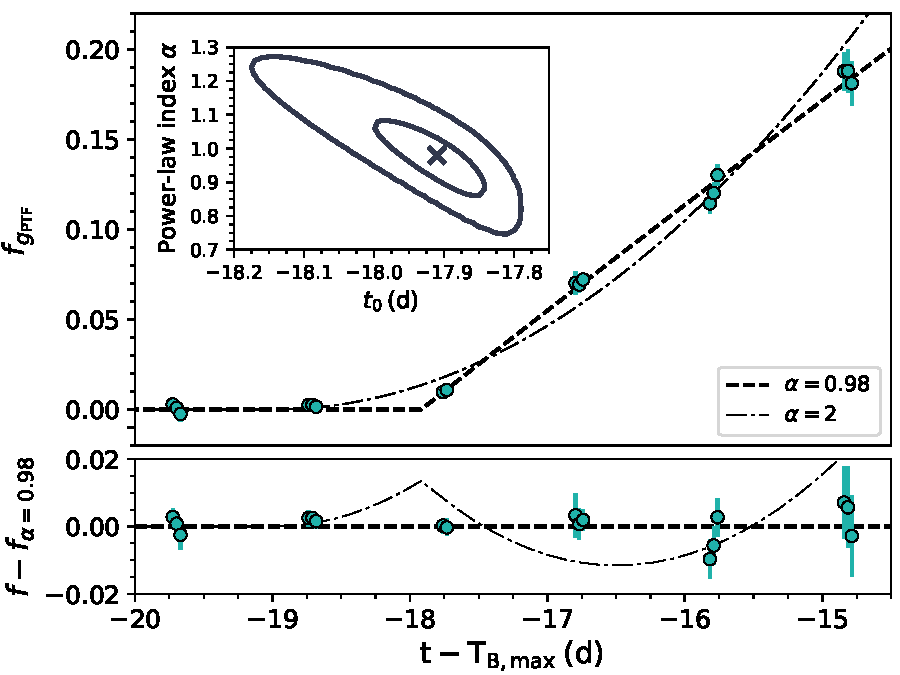
\includegraphics[width=0.95\textwidth]{early_lc.pdf}
  \caption{Broken Power low fitting to the early $g$-band light
    curve. The best-fit model of $\alpha=0.92$ and $t_0=-18.47\,\textrm{days}$
    and corresponding residues are shown in the top and bottom panels, respectively.
    The joint distribution of $t_0$ and $\alpha$ is illustrated in the inset of
    the upper panel. The solid and dashed contours represent the $68\%$ and $99.7\%$
    confidence levels.
  }
  \label{fig:early_lc_fit}
\end{figure*}

Starting from $t=-15\,\textrm{days}$, the \textit{g}-band light curve
rises significantly faster than the best-fit model above, indicating a
greater value of the power-law index $\alpha$. In fact, the light
curve between $t=-14$ and $t=-8$\,days can be fitted with another
power law of index $1.40$. In another word, the whole light curve
before $t=-8$\,days can be approximated by a broken power-law model
(e.g.,
\citealt{2013ApJ...778L..15Z,2014ApJ...783L..24Z,2016arXiv161202097Z,
  2016arXiv161202725Z}).

As discussed in Section \ref{sec:lc_energy}, the initial light curve
of iPTF16abc is probably purely powered by radioactive decay of
$^{56}$Ni. Therefore, the initial rise of the light curve depends on
the depth of the shallowest layer where $^{56}$Ni is deposited
\citep{2014ApJ...784...85P}. According to theoretical mdels
\citep{2016ApJ...826...96P}, the linearly rising light curve implies
strong mixing of $^{56}$Ni in the ejecta. As a result, the time lag
between the SN explosion and the initial rise of the radioactively
powered light curve is negligible.

\subsection{Expansion Velocity Fit}
\label{sec:early_vel}

In order to constrain the explosion time of the SN independently of
the SN light curve, \citet{2014ApJ...784...85P} suggested to measure
the expansion velocities of the photosphere, because the expansion of
the ejecta starts at the onset of the SN explosion. Assuming a
constant opacity in the ejecta, the photospheric velocity evolves as
$v_{ph}\propto(t-t_{exp})^{-0.22}$. While the photospheric velocities
are not easy to measure, line velocities of \ion{Si}{2} or \ion{Ca}{2}
are usually used to approximate the photospheric velocities
\citep{2014ApJ...784...85P,2016ApJ...826..144S}.

In the case of iPTF16abc, the \ion{Ca}{2} IR triplet is very weak in
the spectra probably due to high temperatures in the ejecta. Thus we
perform our measurements on the \ion{Si}{2}\,6355 line. Visual
inspection of the spectra shows no sign of multi-velocity components
of \ion{Si}{2}, and that the \ion{C}{2}\,6580 line overlaps the red
wing of the \ion{Si}{2} line. Consequently we apply a mathematical
model of two gaussian kernels superposed on a linear term, which
accounts for the absorption of \ion{Si}{2} and \ion{C}{2} and the
continuum component, respectively, to approach the observed spectra
between $5,900$ and $6,500$\,\AA (rest-frame). The expansion
velocity of \ion{Si}{2} is calculated at the central wavelength
of the \ion{Si}{2} Gaussian kernel.

\begin{figure*}[!thb]
  \centering
  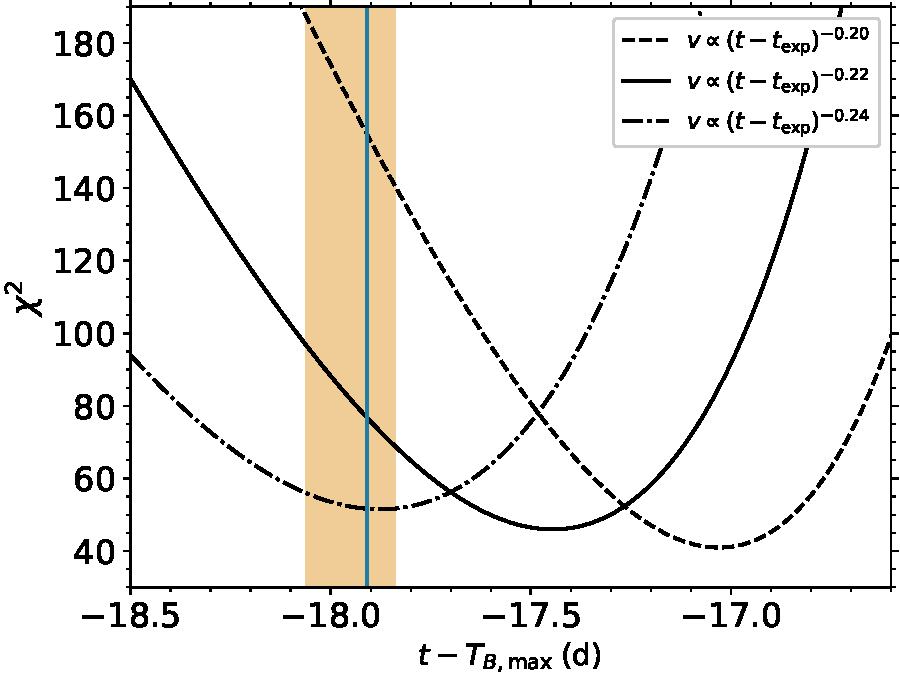
\includegraphics[width=0.45\textwidth]{Chi2.pdf}
  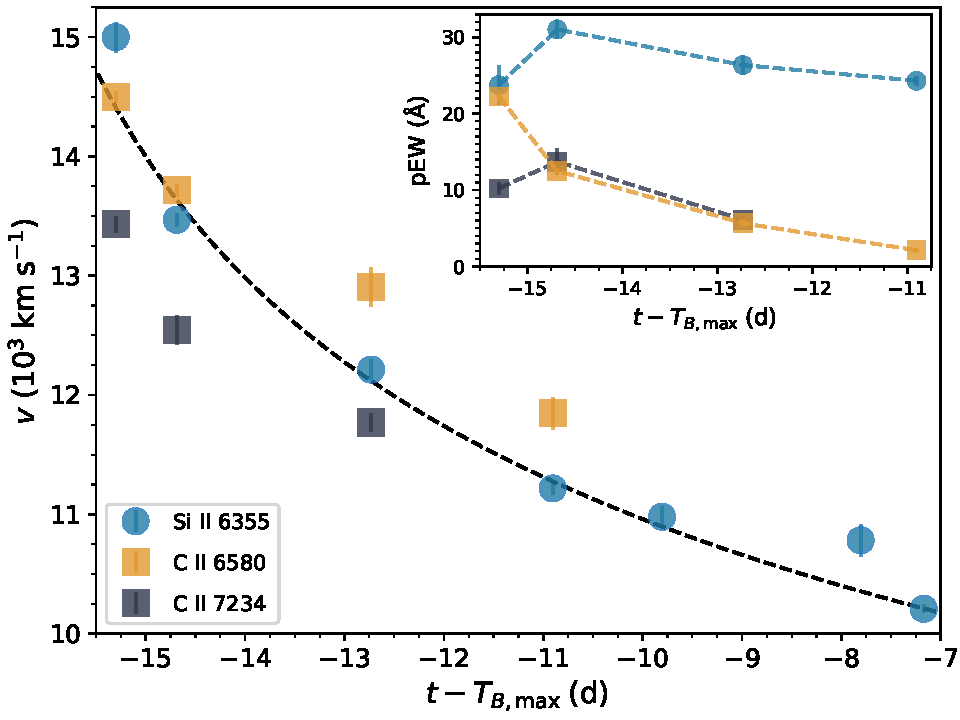
\includegraphics[width=0.45\textwidth]{VelocityPlot.pdf}
  \caption{Constraints on $t_{exp}$ from fitting the velocity
    evolution of \ion{Si}{2}.
    \textit{Left panel:} the dashed, solid
    and dash-dotted curves show $\chi^2$ for fitting power laws with
    indices $-0.20$, $-0.22$ and $-0.24$, respectively. The red
    vertical line and the orange region indicate $t_0$ and its
    3-$\sigma$ confidence interval from Section
    \ref{sec:lc_fit}.
    \textit{Right panel:} Observed \ion{Si}{2}\,6355
    velocities and the best-fit power-law velocity with an index of
    $-0.22$.}
  \label{fig:velocity_t_exp}
\end{figure*}

We fit the measured velocities of \ion{Si}{2}\,6355 line to the
$v\propto(t-t_{exp})^{-0.22}$ model by minimizing the $\chi^2$ value
and find the best-fit explosion time $t_{exp}=-17.95\,\textrm{days}$
with a 3-$\sigma$ confidence interval between $-17.4\,\textrm{days}$
and $-18.3\,\textrm{days}$ (Figure \ref{fig:velocity_t_exp}). We also
alter the power-law index to $-0.20$ and $-0.24$ to examine how
sensitively the result depends on the assumed power-law index.  we
find consistent results within respective 3-$\sigma$ confidence
intervals.

Keeping in mind that $t_{exp}$ has a very large uncertainty mostly due
to the assumption in the $v\propto(t-t_{exp})^{-0.22}$ model, we
compare the estimated $t_{exp}$ to $t_0$ (left panel of Figure
\ref{fig:velocity_t_exp}) and find that $t_0\lessapprox t_{exp}$.
Since physical causality requires $t_{exp}<t_0$, we draw a qualitative
conclusion that $t_0\simeq t_{exp}$. This conclusion is consistent
with our inference from the early light curve analysis in Section
\ref{sec:lc_fit}.

With $t_{exp}$, we estimate the actual rise time of iPTF16abc from the
SN explosion to its \textit{B}-band maximum to be $17.95$ days.  In
comparison, SN2011fe has $t_0=-17.7$ days \citep{2013A&A...554A..27P}
with a preceding dark period of $\sim 1$ day
\citep{2014ApJ...784...85P}. ASASSN-14lp has $t_0=-16.94$ days with a
preceding dark period of about acouple of days
\citep{2016ApJ...826..144S}. This comparison suggests that the actual
rise time of a SN Ia between the SN explosion and the \textit{B}-band
maximum is roughly a constant, which largely depends on the total mass
of synthesized $^{56}$Ni. 

\subsection{Strong and Short-Lived Carbon Features}
\label{sec:carbon}

Another intriguing spectral feature of iPTF16abc is strong absorption of
\ion{C}{2}\,6580 and \ion{C}{2}\,7234 lines. Our analysis on the
\ion{Si}{2}\,6355 line also allows us to measure the velocities and
pseudo-equivalent widths (pEWs) of \ion{C}{2}\,6580. We also fit a Gaussian
kernel superposing on a linear term to the spectral region near
the \ion{C}{2}\,7234 line to measure its velocity and pseudo-equivalent
width. The velocity evolution of \ion{C}{2} is shown in the right panel
of Figure \ref{fig:velocity_t_exp} and the pEW evolution
in Figure \ref{fig:ew}. 

Our measurements show that the strong \ion{C}{2} absorption
only appears in the very early phases. In the spectrum taken at
$t=-15.8$ days, the pEW of \ion{C}{2}\,6580 is comparable to that
of \ion{Si}{2}\,6355. Then the pEW of \ion{C}{2} decreases
until they disappear at about $t=-10$ days. 

\begin{figure}[!htb]
  \centering
  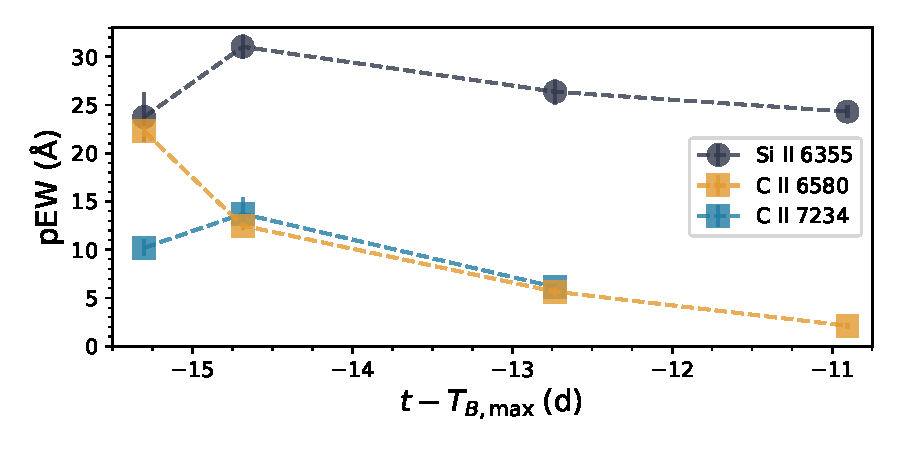
\includegraphics[width=0.45\textwidth]{pEW.pdf}
  \caption{Pseudo-equivalent width of \ion{Si}{2}\,6355,
    \ion{C}{2}\,6580 and \ion{C}{2}\,7234 lines. The uncertainties
    in these measurements are less than the sizes of these symbols.}
  \label{fig:ew}
\end{figure}

Formation of \ion{C}{2} absorption requires existence of both unburned
carbon and $^{56}$Ni, the latter of which is responsible to ionize the
carbon atoms. The strong and short-lived \ion{C}{2} features observed
in the spectra of iPTF16abc show that a certain amount of carbon atoms
exist in the outer layers of the ejecta and that $^{56}$Ni atoms are also
strongly mixed in the same layers. This provides a third piece of evidence
to strong mixing in the iPTF16abc ejecta. 

Carbon signatures are seen in over $1/4$ of all normal SNe Ia before
maxima
\citep{2011ApJ...732...30P,2012MNRAS.425.1917S,2011ApJ...743...27T},
but the signatures are usually weak. Even in SN2011fe, the \ion{C}{2}
features are not strong in the first spectra
\citep{2012ApJ...752L..26P}.  The only normal SN Ia known to have
strong \ion{C}{2} features at early phases is SN2013dy
\citep{2013ApJ...778L..15Z}. Unlike iPTF16abc, however, the equivalent
widths of \ion{C}{2} features in SN2013dy are as large as those of
\ion{Si}{2}\,6355 in the same spectra.


\subsection{Discussions}
\label{sec:lc_energy}

Early radiation of a SN Ia may have multiple energy sources: SN shock
breakout, SN-companion collision, and radioactive activity. The
previous analysis is based on the assumption that the light curve of
iPTF16abc is powered purely by radioactive decay. Here we discuss the
other two possibilities.

\subsubsection{SN Shock Breakout}

The shock breakout of a SN Ia lasts for a fraction of a second due to
the small size of the exploding star. However, the subsequent cooling
phase may last longer (e.g., \citealt{2010ApJ...708..598P}).
Following the analysis of SN2011fe in \citet{2012ApJ...744L..17B}, we
compare the early-phase \textit{g}-band light curve of iPTF16abc with
two cooling models \citep{2011ApJ...728...63R, 2010ApJ...708..598P}
and reach a not very constraining conclusion that the radius of the
progenitor star of iPTF16abc should be $<1\sr$. In fact, with a
typical $0.01\sr$ radius of a white dwarf, the cooling emission of a
SN Ia is negligible at the time of the first detection of iPTF16abc.

\subsubsection{SN-Companion collision}

From a SN Ia born in a single-degenerate system, with an odd of
$\lesssim10\%$ due to the geometry, we expect to see emission produced
by SN ejecta slamming into the companion. According to calculations by
\citet{2010ApJ...708.1025K}, collision between SN ejecta and the
companion star generates thermal emission with a spectrum with
spectrum that peaks in the ultraviolet. The Rayleigh-Jeans tail
emission in the \textit{g} band is very weak.

In order to examine the possible SN-companion signature in the early
light curve of iPTF16abc, we employ the \citet{2010ApJ...708.1025K}
model by assuming an ejecta mass of $1.4\sm$, an expansion velocity of
$10^{4}\,\textrm{km}\,\textrm{s}^{-1}$, and a constant opacity of
$0.2\,\textrm{cm}^2\,\textrm{g}^{-1}$. The angular dependence of this
emission uses the parameterized equation in
\citet{2012ApJ...749...18B}.  Figure \ref{fig:SN-companion} compares
the calculated \textit{g}-band apparent magnitudes of SN-companion
collision for different combinations of binary separation and viewing
angle against the first detection of iPTF16abc. The figure shows that,
even with the most favored viewing angle, the binary separation would
have to exceed $2\times10^{14}\,\textrm{cm}$. Under the model assumption that the
companion fills its Roche lobe, the companion star would have to have
a radius of $\sim10^{14}\,\textrm{cm}\simeq10^{4}\sr$. Given that the
mass of the companion is $\sim1\sr$, such a large radius seems unlikely.
Therefore, we conclude that the early emission of iPTF16abc is not likely
to originate from the SN-companion collision. 

\begin{figure}[!thb]
  \centering
  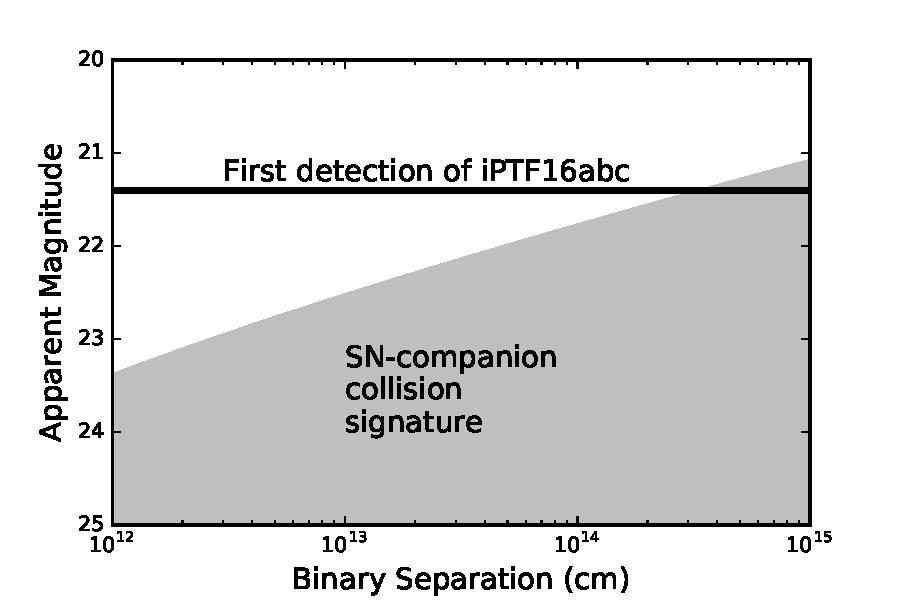
\includegraphics[width=0.45\textwidth]{SNCompanion.pdf}
  \caption{apparent magnitude of SN-companion collision (gray region)
    against the first detection of iPTF16abc (black).}
  \label{fig:SN-companion}
\end{figure}

\section{Conclusion}
\label{sec:conclusion}

In this paper, we present observations of an extraordinarily young
normal Type Ia supernova iPTF16abc at one tidal tail of NGC\,5221. Our
extraordinarily fast-response follow-up compaign of this supernova
allows us to draw the following conclusions:
\begin{itemize}
\item By extrapolating the early light curve, we determine that the
  first light of the SN light curve was only $0.18$ days before our
  first observation.
\item Our analysis shows that the observed early-phase light curve is
  probably powered by radioactive decay of $^{56}$Ni, instead of SN
  shock breakout or SN-companion collision (provided that iPTF16abc
  is born in a single-degenerate channel).
\item Our measurements on the spectral line velocities shows that the
  actual explosion date of the SN is approximately equal to the time
  of the first light of the SN light curve, indicating that
  synthesized $^{56}$Ni atoms are mixed out into the outer layers of
  the supernova ejecta.
\item The strong mixing of $^{56}$Ni is also supported by strong and
  short-lived carbon features in the earliest spectra of iPTF16abc. 
\end{itemize}

Observations of extraordinarily young supernovae provide a ``smoking
gun'' to probe the mixing level in the ejecta, which, in turn, results
directly from the explosion mechanisms. With the ongoing and planned
time-domain survyes, a large number of extraordinarily young supernovae
will be collected in the next few years. With such a sample, we will
be able to make connections between the observed supernovae and proposed
mechanisms.

It should also be emphasized that much of the analysis presented in
this paper would not be possible without the fast-response and
extensive photometric and spectroscopic follow-up compaign. With the
great potential of discoveries in the surveys, researchers need to
be prepared and organized for follow-up observations. 

\acknowledgements

YC thanks supports from the postdoc fellowship in the eScience
institute, University of Washington.

\bibliographystyle{aasjournal}
\bibliography{ref}

\end{document}
